\documentclass[../../syllabus_1.tex]{subfiles}
\begin{document}

\chapter{Calcul littéral}

%\faIcon{book} Théorie pages 73 à 77

\section*{Matières}
\begin{enumerate}[label=\textbf{\arabic*.}]
    \item Vocabulaire dans le calcul littéral
    \item Valeur numérique d’une expression algébrique
    \item Les familles de nombres
    \item Réduire une somme algébrique
    \item Réduire un produit algébrique
    \item Suppression des parenthèses
\end{enumerate}

\section{Une nouvelle facçon de penser}
Pendant des milliers d'années, les hommes ont appris à compter. Ils comptaient leurs moutons, leurs sacs de blé, leurs pièces d'or ou encore les pierres nécessaires pour construire une maison. Les mathématiques servaient surtout à répondre à une question très simple :
« Combien y en a-t-il ? ».

Mais, petit à petit, les problèmes sont devenus plus compliqués. Parfois, on ne connaissait pas encore le nombre recherché. Par exemple, un marchand savait qu'il devait partager sa récolte entre plusieurs personnes, mais il ne connaissait pas encore la quantité exacte de blé. Un architecte savait qu'il devait construire une porte deux fois plus haute que sa largeur, sans connaître les dimensions à l'avance. Un commerçant voulait prévoir le bénéfice qu'il ferait selon le nombre d'objets vendus. Les mathématiques devaient donc apprendre à parler de quantités inconnues.

Au début, les savants écrivaient de longues phrases pour décrire ces quantités. Les Babyloniens et les Égyptiens résolvaient déjà ce genre de problèmes il y a près de $4 000$ ans, mais ils n'avaient ni lettres, ni symboles particuliers.
Les Grecs, eux, préféraient représenter ces quantités avec des figures géométriques. Pour eux, un nombre pouvait être imaginé comme la longueur d'un segment ou la surface d'un carré.

Puis, vers l'an 820, un grand mathématicien nommé Al-Khwarizmi rassembla toutes ces méthodes dans un livre appelé « Al-jabr », un mot arabe qui signifie « remettre ensemble » ou « réparer ». C'est de ce mot que vient le mot algèbre. Mais la véritable révolution arriva plusieurs siècles plus tard.

Des mathématiciens eurent une idée très simple :
« Et si, au lieu de toujours écrire de longues phrases, on utilisait une lettre pour représenter un nombre, même si on ne le connaît pas encore ? ». Cette idée changea complètement les mathématiques.

Grâce aux lettres, on pouvait décrire une infinité de situations différentes avec une seule écriture. Plus besoin de connaître les nombres à l'avance : on pouvait réfléchir de manière générale. C'est exactement ce que fait l'algèbre. L'algèbre n'est donc pas seulement une manière de calculer. C'est un nouveau langage qui permet de parler de nombres connus... mais aussi de nombres inconnus, de quantités qui changent ou de situations que l'on veut prévoir.

L'arithmétique répond à la question : « Combien ? ». L'algèbre répond à la question : « Et si je ne connais pas encore le nombre ? ».
C'est un peu comme la différence entre raconter une seule histoire et écrire une recette qui fonctionne pour toutes les histoires. L'algèbre ne s'intéresse plus seulement aux nombres, mais aux relations entre les nombres. C'est cette idée qui en fait l'un des langages les plus puissants des mathématiques.

\section{Exploration}
L'algèbre consiste à travailler avec des nombres et avec des lettres. Les lettres peuvent représenter n'importe quel nombre, ce qui permet de calculer de façon beaucoup plus rapide et puissante !

En fait, tu connais déjà des calculs avec des lettres. Indique des exemples.

\vspace{2cm}

Quelle est l’utilité de l’utilisation des lettres dans ces exemples ?

\vspace{2cm}

Imagine la construction d'un immeuble qui compte 3 fenêtres à chaque étage Combien l'architecte doit-il prévoir de fenêtres si le bâtiment compte :\\
7 étages :\\
21 étages :\\
1000 étages :\\

\newpage
\section{Vocabulaire}

Une expression algébrique (ou expression littérale) est une expression dans laquelle se mêlent des nombres et des lettres. Chaque terme se compose d'un \textbf{coefficient} et d'une \textbf{partie littérale}.

\begin{center}
    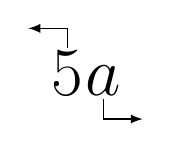
\begin{tikzpicture}[>=latex, line width=0.5pt]
        \begin{Huge}
            \draw (0,0)node[inner sep=1pt, anchor=south,name=A]{\(5\)};
            \draw (1.2ex,0)node[inner sep=1pt, anchor=south,name=B]{\(a\)};
            \draw[->] (A.north) --++(0,0.25) --++(-0.5,0);
            \draw[->] (B.south) --++(0,-.25) --++(0.5,0);
        \end{Huge}
    \end{tikzpicture}
\end{center}

\begin{center}
    
\includegraphics[]{chapitres/calcul_litteral/img/einstein1.png}
\end{center}

Pour alléger les expressions algébriques, on peut supprimer le signe de la multiplication (\(\cdot\)) entre :
\begin{itemize}
    \item un nombre et une lettre (un coefficient et une partie littérale) : \(3 \cdot a = 3a \)
    \item deux lettres (deux facteurs littéraux) : \(a \cdot b = ab \)
    \item un facteur et une parenthèse : \(2 \cdot (a+b) = 2(a+b) \)
    \item deux parenthèses : \((a+c) \cdot (b+d) = (a+c) (b+d) \)
\end{itemize}

Remarque : 
\begin{itemize}
    \item \(a = 1 \cdot a \) (le coefficient est $1$, mais on ne l'écrit pas)
    \item \(-a = -1 \cdot a \) (le coefficient est $-1$, mais on ne l'écrit pas)
    \item \(0 \cdot a = 0 \)
\end{itemize}

\begin{exercise}
    Applique les conventions correctement dans les expressions algébriques suivantes.
    \begin{enumerate}[cols=2]
        \item \(4 \cdot a + b = \)
        \item \(y \cdot x \cdot 9 = \)
        \item \(1 \cdot b + 1 \cdot c = \)
        \item \(5 \cdot b - 1 \cdot x = \)
        \item \(0 \cdot a = \)
    \end{enumerate}
\end{exercise}

\begin{exercise}
    Complète les phrases ci-dessous en utilisant le vocabulaire adéquat. %\FIXME: mise en page pour réponses
    \begin{enumerate}[itemsep=.5cm]
        \item \(a + b + c\) est une \dotfill de trois \dotfill
        \item \(abc\) est un \dotfill de trois \dotfill
        \item \(b^{3}\) est une \dotfill, elle peut s'écrire sous la forme d'un \dotfill \\ de trois \dotfill égaux (= \dotfill). \(b^3\) est le \dotfill de \(b\).
        \item \(3b\) est un \dotfill. \(3\) est le \dotfill de \(b\). \(3b\) est le \dotfill de \(b\).
    \end{enumerate}
    \vspace{.5cm}
\end{exercise}

\newpage
\section{Valeurs numériques d'une expression algébrique}

Calculer la valeur numérique d'une expression consiste à remplacer les lettres (appelées variables) par des nombres donnés et à effectuer les opérations.
\begin{equation*}
    8a+5
\end{equation*}
Calculer sa valeur numérique pour \(a = 2\) revient à remplacer \(a\) par \(2\) dans l'égalité de départ et à respecter les priorités des opérations pour calculer le résultat.

Ici, cela nous donne,
\begin{align*}
    8 \cdot 2 + 5 & = 16 + 5 \\
                  & = 21
\end{align*}
N’hésite pas à mettre les multiplications en évidence en rajoutant le symbole \(\cdot \) avant de remplacer les lettres par leurs valeurs numériques.
N’oublie pas de mettre les nombres négatifs entre parenthèses.

\begin{exercise}
    Calcule la valeur numérique des expressions algébriques ci-dessous.
    \begin{enumerate}[itemsep=3cm, cols=2]
        \item \(3t + 5t^{2}\) \quad pour \(t = 6\).
        \item \(x^{2} + 3x - 10\) \quad pour \(x = - 3\).
        \item \(10b-5\) \quad pour \(b=12\).
        \item \(a^2-1\) \quad pour \(a=-2\).
        \item \(ab+2\)\quad pour \(a=-7\) et \(b=-8\).
        \item \(2a+3b-1\) \quad pour \(a=-25\) et \(b=9\).
        \item \((a+2b)\cdot 3\) pour \(a=-3\) et \(b=-2\).
        \item \(\left(a^2 - 3ab\right)^2\) pour \(a=-1\) et \(b=0\).
    \end{enumerate}
    \vspace*{3cm}
\end{exercise}

\newpage

\begin{exercise}
    Code chaque phrase ci-dessous par une expression algébrique.
    \begin{enumerate}[cols=2, itemsep=2cm]
        \item La somme de \(a\) et de \(b\)
        \item Le produit de \(c\) par \(d\)
        \item La somme de \(a\) et du double de \(b\)
        \item Le carré de \(a\)
        \item Le carré de la somme de \(x\) et de \(y\)
        \item Le produit de \(c\) par le cube de \(d\)
        \item L'opposé de \(b\)
        \item Le triple du produit de \(x\) par \(y\)
    \end{enumerate}
\end{exercise} 

\section{Les familles de nombres}

Un nombre naturel peux être désigné par la lettre \(n\). Nous pouvons utiliser l'expression littérale pour représenter des familles de nombres.

\begin{center}
    \begin{tblr}{
            hlines,
            vlines,
            rows={1.4cm,m},
            columns={0.5\linewidth},
            row{1}={font=\bfseries, 1cm},
        }
        Écriture générale & Exemple chiffré \\
         Un multiple de \(3\) s'écrit \(3n\) & 12 est un multiple de 3, car \(12=3\cdot 4\) \\
         Un multiple de \(10\) s'écrit \(10n\) & 30 est un multiple de 10, car \(30 = 10 \cdot 3\) \\ 
        Un multiple de \(2\) ou un nombre pair s'écrit \(2n\) & 10 est un nombre pair, car \(10 = 2\cdot 5\) \\
         Un nombre impair s'écrit \(2n+1\) & 11 est un nombre impair, car \(11=2\cdot 5+1\) \\
         Deux nombres consécutifs s'écrivent \(n\) et \(n+1\) & 14 et 15 sont des nombres consécutifs, car 15 = \(14+1\) \\
         Trois nombres consécutifs s'écrivent \(n\), \(n+1\) et \(n+2\) & 25, 26 et 27 sont trois nombres consécutifs, car \(26=25+1\) et \(27 = 25 +2\)\\
    \end{tblr}
\end{center}

\newpage
\section{Réduire une somme algébrique}
\begin{center}
    
\includegraphics[width=10cm]{chapitres/calcul_litteral/img/einstein2.png}
\end{center}

\dotsforanswer{2}[Des termes semblables sont]
\exemples
\vspace{4cm}
%\FIXME: refaire ces petites synthèses en plus joli

Comment réduire une somme algébrique ?

Pour additionner des termes semblables, il suffit :
\dotsforanswer{3}
%\begin{itemize}
%    \item d'additionner les coefficients.
%    \item de conserver (recopier) la partie littérale.
%\end{itemize}
\vfil
\exemples
\begin{enumerate}[cols=2, itemsep=1cm, label=]
    \item \(3a+5a=\)
    \item \(7ab-11ab=\)
    \item \(2x^3 + x^3=\)
    \item \(3a^2 + 5a=\)
\end{enumerate}

\begin{exercise}
    Réduis au maximum les expressions suivantes.
    \begin{enumerate}[cols=3, itemsep=1cm]
        \item \(7a - 5a =\)
        \item \(3a + 7a =\)
        \item \(- 2b + 8b =\)
        \item \(- 3a + a =\)
        \item \(5a + 7 - 6b - 10 =\)
        \item \(3x + 2x - 8 - 7x =\)
    \end{enumerate}
\end{exercise}

\newpage
\begin{exercise}
    Réduis, si possible, les expressions suivantes.
    \begin{enumerate}[cols=2, itemsep=1cm]
        \item \(3 + 7a - 8 =\)
        \item \(3x + 2y =\)
        \item \(4a^{2} - 8a^{2} =\)
        \item \(- c + 3c =\)
        \item \(7a - 7x =\)
        \item \(- 3 + 5 + x - 7x =\)
        \item \(4x^{2} + 5x =\)
        \item \(10a + 5b - 13b - 6a =\)
    \end{enumerate}
\end{exercise}

\begin{exercise}
    Réduis, si possible, les expressions suivantes.
    \begin{enumerate}[cols=2, itemsep=1cm]
        \item \(5a^{2} + 10a^{2} =\)
        \item \(25b + ( - 8b) =\)
        \item \(7a + 3b =\)
        \item \(a^{3} - ( - 7a^{3}) =\)
        \item \(x + 5 + 2x =\)
        \item \(- 2b + 4b =\)
        \item \(4 + a + 4 + a² + 2a =\)
        \item \(- 3 + x + ( - 5) =\)
        \item \(a + 4a - 8 - 5 - a =\)
        \item \(2y+3x-5x-20y=\)
    \end{enumerate}
\end{exercise}

\newpage
\section{Réduire un produit algébrique}
Comment réduire un produit algébrique ?

Pour réduire un produit algébrique, il suffit de :
\dotsforanswer{3}
%\begin{itemize}
%    \item multiplier les coefficients entre eux
%    \item multiplier les facteurs littéraux entre eux.
%\end{itemize}

\exemples
\begin{enumerate}[cols=2, itemsep=0.8cm, label=]
    \item \(3a\cdot 5a=\)
    \item \(7a \cdot (-3b)=\)
    \item \(a\cdot a\cdot a\cdot a=\)
    \item \(-5x\cdot 3y=\)
\end{enumerate}

\begin{exercise}
    Réduis les produits suivants.
    \begin{enumerate}[cols=2, itemsep=0.8cm]
        \item \(a \cdot a \cdot a =\)
        \item \(c \cdot 2c =\)
        \item \(2a \cdot 2ab =\)
        \item \(2e \cdot e \cdot e \cdot 3e =\)
        \item \(x \cdot x \cdot x^{3} =\)
        \item \(e \cdot ef \cdot e^{2} \cdot f^{5} =\)
        \item \(5x\cdot 3x=\)
        \item \(-8a\cdot 2a=\)
        \item \(-4x^2y \cdot (-2x)=\)
        \item \(2x\cdot 3x \cdot 2x=\)
    \end{enumerate}
\end{exercise}

\begin{exercise}
    Réduis au maximum les expressions algébriques ci-dessous.
    \begin{enumerate}[cols=2, itemsep=0.8cm]
        \item \(4a \cdot 2b =\)
        \item \(- 2a \cdot ( - 3b) =\)
        \item \(2a \cdot ( - 5b) =\)
        \item \(3a \cdot 2a =\)
        \item \(- 2b \cdot 3b =\)
        \item \(- 4c \cdot ( - 2c) =\)
        \item \(3a \cdot b =\)
        \item \(- 2a \cdot ( - 5a) \cdot ( - 3a) =\)
    \end{enumerate}
\end{exercise}

\newpage
\begin{exercise}
    Réduis au maximum les expressions suivantes.
    \begin{enumerate}[cols=2, itemsep=.7cm]
        \item \(- 3 \cdot 2a =\)
        \item \(- 5x \cdot ( - 2x) \cdot 3x =\)
        \item \(- 3a + 2a =\)
        \item \(- 2a - 4b =\)
        \item \(- 8a + a =\)
        \item \(5x \cdot ( - 2x) =\)
        \item \(- 4c - 2c =\)
        \item \(- 3 \cdot ( - 2a) \cdot a =\)
        \item \(- 3a² - 2a² + a² =\)
        \item \(- 3a + 2a² - 4b + 12b =\)
        \item \(- a \cdot a =\)
        \item \(3 + 6b - 7b + 12 =\)
    \end{enumerate}
\end{exercise}

\begin{exercise}
    Réduis au maximum les expressions suivantes. Attention à la priorité des opérations.
    \begin{enumerate}[cols=2, itemsep=2cm]
        \item \(- 2c \cdot 3d + 3c \cdot d =\)
        \item \(2a \cdot 3a + 5a \cdot ( - 2a) =\)
        \item \(- a + 2 \cdot a \cdot ( - 3) =\)
        \item \(4x \cdot 3x \cdot x - 2x \cdot 6\cdot x^2 =\)
        \item \(- 6 \cdot ( - 4a) - 2 \cdot 3a =\)
        \item  \(2b \cdot 3a - 2ab =\)
        \item \(5a + 3 \cdot 2a - 5 \cdot 6a=\)
        \item \(\left(5a \cdot 5ab + 5a^2b\right) + 6a^2b=\)
        \item \(-8x\cdot 2x - (-2 \cdot 3x^2)=\)
        \item \(2a \cdot 7b - 10ab + 6b \cdot (-2a)=\)
    \end{enumerate}
\end{exercise}

\newpage
%\section{Distributivité simple}
%
%Souviens-toi de la distributivité simple. Quel procédé utilise-t-on pour calculer facilement \(7 \cdot 16 \) ?
%
%\vspace{4cm}
%
%\begin{exercise}
%    Calcule en utilisant la distributivité simple.
%    \begin{enumerate}[itemsep=3cm]
%        \item \(23 \cdot 6 =\)
%        \item \(72 \cdot 11 =\)
%        \item \(26 \cdot 9 =\)
%        \item \(101 \cdot 27 =\)
%    \end{enumerate}
%    \vspace{3cm}
%\end{exercise}
%
%La même méthode s'utilise dans le calcul algébrique.
%
%\(a\cdot (b+c)=\)
%
%\newpage
%\textbf{Remarque}
%
%\begin{exercise}
%    Réduis au maximum les expressions algébriques suivantes en utilisant la distributivité simple.
%    \begin{enumerate}[cols=2, itemsep=1cm]
%        \item \(3 \cdot (2a + 4b) =\)
%        \item \((4x - 2y) \cdot 2 =\)
%        \item \(a \cdot (a + b) =\)
%        \item \(-2y(3y - 5x) =\)
%        \item \(10(a - 3x) =\)
%        \item \(- 2a(4b - 3c) =\)
%        \item \((3 + 2x) \cdot 2x =\)
%        \item \((3b - 5) \cdot 4x =\)
%    \end{enumerate}
%    \vspace{1cm}
%\end{exercise}
%
%\begin{exercise}
%    Exprime l'aire de la figure suivante de plusieurs manières à l'aide d'une expression littérale. \\
%    
\includegraphics{chapitres/calcul_litteral/img/distrib..png}
%\end{exercise}
%
%\newpage
%\begin{exercise}
%    Réduis au maximum les expressions suivantes.
%    \begin{enumerate}[itemsep=3cm]
%        \item \(3x^{2} + 2\left( 5x^{2} - 7 \right) =\)
%        \item \(- 5(3a + 2b) + 5a \cdot 7b =\)
%        \item \(- 10x \cdot 2x + (8x + 2) \cdot 3x =\)
%        \item \((8a - 7b)\cdot 2 + 5a\left(-3-2b\right)=\)
%        \item \(-x\left(7-x\right) - 2(x^2 +x)=\)
%    \end{enumerate}
%    \vspace{2.5cm}
%\end{exercise}
%
%\newpage
%\section{Factoriser par la mise en évidence}
%\dotsforanswer{2}[Factoriser une expression, c'est]
%
%\vspace{4cm}
%
%\begin{exercise}
%    Factorise au maximum les sommes algébriques suivantes, à l'aide de la mise en évidence.
%    \begin{enumerate}[cols=2, itemsep=1cm]
%        \item \(3a + 3b =\)
%        \item \(6a - 7ab =\)
%        \item \(15bd + 7ad =\)
%        \item \(5xy + 5x =\)
%        \item \(8ax + 2am - 4axm =\)
%        \item \(a^3b^9 - a^6b^2c =\)
%    \end{enumerate}
%    \vspace{1cm}
%\end{exercise}
%
%\begin{exercise}
%    Factorise au maximum en utilisant la mise en évidence.
%    \begin{enumerate}[cols=2, itemsep=1.5cm]
%        \item \(6a + 12b =\)
%        \item \(15x + 5y =\)
%        \item \(3x + 9y =\)
%        \item \(20ab - 24a =\)
%        \item \(3a^3x^2 + 6a^3x^6  - 15 a^5x^2 =\)
%        \item \(42xy + 12y =\)
%    \end{enumerate}
%    \vspace{1.5cm}
%\end{exercise}

\newpage
\section{Suppression de parenthèses}
Quelle sont les règles à respecter lorsqu'on veut retirer des parenthèses~?

\dotsforanswer{2}[Si la parenthèse est précédée d'un signe \(" + "\) : ]
\exemples
\begin{enumerate}[itemsep=1.5cm, cols=2, label=]
    \item \(15 + (5a - 9) =\)
    \item \(2a + (10a + 2b) =\)
    \item \(3x + ( - 5x - 2) =\)
    \item \(2x + (5-3x)=\)
\end{enumerate}
\vspace{1.5cm}

\dotsforanswer{2}[Si la parenthèse est précédée d'un signe \(" - "\) :]
\exemples
\begin{enumerate}[itemsep=1.5cm, cols=2, label=]
    \item \(15 - (5 - 9a) =\)
    \item \(2a - (8a + 8b) =\)
    \item \(3x - (7x - 2) =\)
    \item \(-(-6x+3) - 1=\)
\end{enumerate}
\vspace{1.5cm}

\begin{exercise}
    Réduis au maximum les expressions suivantes après avoir supprimé les parenthèses.
    \begin{enumerate}[cols=2, itemsep=2cm]
        \item \(9d+(8d-1)+3=\)
        \item \(a^2 - (6b-3a^2)=\)
%        \item \(2(5x + 3y) - 3y = \)
        \item \(-(2x+3y) + (5+9x)=\)
    \end{enumerate}
\end{exercise}

\newpage
\section{Exercices mélangés}
\setcounter{exercise}{0}

\begin{exercise}
    Réduis si possible les expressions suivantes, sinon recopie-les.
    \begin{enumerate}[cols=3, itemsep=.6cm]
        \item \(2a + 3a \)
        \item \(2m\cdot3n \)
        \item \(3a\  + a \)
        \item \(4a\cdot3b \)
        \item \(\ 6x\cdot5x\  \)
        \item \(3a\cdot2a \)
        \item \(- \ 5m + 2y \)
        \item \(3t\cdot( - 2t) \)
        \item \(x\cdot3y \)
        \item \( m - m \)
        \item  \(m - 3m \)
        \item \(8x - 2x \)
        \item \(6x\cdot5y \)
        \item \(5y\cdot y \)
        \item \(3ab - \ 5ab \)
        \item \(5a^2  + \ 15 \)
        \item \(- 9mp\cdot4n \)
        \item \(23l \cdot 4mp \)
        \item \(4b\cdot4b \)
        \item \(\ 12b\cdot5l\  \)
        \item \(9ab\cdot2s \)
        \item \(m + m^{2} \)
        \item \(30\ \cdot\ 10a \)
        \item \(2v\ \cdot\ 3l \)
        \item \( a^5 - 2a \)
        \item \(4i - 2i \)
    \end{enumerate}
\end{exercise}

\begin{exercise}
    Réduis au maximum.
    \begin{enumerate}[cols=2, itemsep=.6cm]
        \item \(3a + 2a - b\)
        \item \(5a + (9 - a)\)
        \item \(10x - (7x + 8)\)
        \item \(5a \cdot 8bc\)
        \item \(15a - 8ab + 9a\)
        \item \(7x + 8y - 10x\)
        \item \((9 - 3a) + (7 + 10a) - ( - 9a - 2)\)
        \item \(- ( - 5 + 3x) + (5x - 12)\)
    \end{enumerate}
\end{exercise}

\newpage
\begin{exercise}
    Réduis au maximum les expressions algébriques suivantes.
    \begin{enumerate}[cols=3, itemsep=.6cm]
        \item \(\ 2b + ( - b + 3)\)
        \item \(-3-(5x+8)\)
        \item \((8a+2b)-(3b-7a)\)
        \item \(- ( - x + y) - ( - y + x)\)
        \item \(3c + ( - a - c)\)
        \item \(8 + (a + 2)\)
        \item \(5a - (7 + 5a)\)
        \item \(d - ( - 2 - d)\)
        \item \(4x - (x - 3)\)
        \item \(x+ (7x-3)+3\)
        \item \(3b + (2b - 9)\)
        \item \(10 - (a - 2 + 5b)\)
        \item \(6a + (2a - 5) - (5a - 7)\)
        \item \(- (c + 3d) + (6d + c)\)
        \item \(4x^{2} + \left( - 2x^{2} - 3 \right)\)
    \end{enumerate}
\end{exercise}

\begin{exercise}
    Réduis au maximum les expressions suivantes. Veille à laisser ton développement visible.
    \begin{enumerate}[cols=2, itemsep=.6cm]
        \item \(2a^{2} + 3a + 2 - 3a²\)
        \item \(4a\ \ \cdot \ \ 3\  - \ 2\ \ \cdot \ \ 3a\)
        \item \(2 \cdot (3a) + 2 \cdot ( - 2a) - ( - 3a + 2)\)
        \item \(- 4a^{2} + 6 - 2a + 3a\)
        \item \(2a\cdot 3b + 4a\cdot 5b \)
        \item \(15x\  + 2x\cdot \ x \)
        \item \(2\cdot 4x^{2} + 5\cdot 3x^{2} \)
        \item \(a^{2}\cdot 3b^{2} - a^{2}\cdot 4b^{2} \)
        \item \(4a\ \ .\ \ 5\  - \ 10a\ \ .\ \ 1\)
        \item \(3a^{2} + 6a - 4 + 3 - 2a^{2}\)
        \item \(2a² - (a² + 10) - ( - 2 + 2a)\)
        \item \((3 + 2a) - ( - 3 - 2a)\)
        \item \(a - a^{2} + 3 + a^{2} - a + 1\)
        \item \(6a - 8a^{2} + 5a^{2} + 6\)
        \item \(3a\ \ .\ \ 3\  + \ 2a\ \ .\ \ ( - 2)\)
        \item \(ab\  + ab\  + 5ab\  + 6a^{2}b \)
        \item \(3a + 5\cdot a\cdot 2 \)
        \item \(3a^{3}\cdot 8 + 2\cdot a\cdot 5a \)
        \item \(8xy\  + (5xy - \ 3xy) \)
%        \item \((3a + 4) \cdot 2a + (3 + a)\)
%        \item \(15ab + 9a(2b + 6) + 5(a + 3ab)\)
%        \item \(7a + (2 + a) \cdot a^{2} + 5a\)
%        \item \(6\  + \ 5\ \cdot \ (\ b\  + 1) \)
%        \item \(5 + 3\cdot \ (x - 2) \)
%        \item \(2\cdot (p + 3) \)
%        \item \(8\cdot (8p - 2q) \)
%        \item \((5x\  + 3y)\cdot \ ( - a)\  \)
%        \item \(4 + 7\cdot ( - 2f + 3) \)
%        \item \(- \ 4\cdot ( - 6 - 7x) \)
%        \item \( 2\cdot (x + 3) + 10x\)
%        \item \(x \cdot (3x - 1) -5x^2 \)
%        \item \(- \ 5c\cdot 2d - 3\cdot d\cdot c \)
%        \item \((6a-b)\cdot (-2b) + 3b^2 \)
%        \item \(3(5x-8)\)
%        \item \(-2x(x-7) - (7x+5)\)
    \end{enumerate}
\end{exercise}

\newpage
\begin{exercise}
    Réduis au maximum les expressions suivantes.
    \begin{enumerate}[cols=2, itemsep=.8cm]
        \item \(5x \cdot 3\)
        \item \(ab\cdot a^3\cdot b^6 \cdot a^2b\)
        \item \(7x-10x\)
        \item \(4\cdot 2x+12x\)
        \item \(5a^2 \cdot 3b - 5a + 3a^2b\)
        \item \(5x \cdot 3x^3 + 10 x^4 - 2x\cdot x \cdot x \cdot (-2x)\)
        \item \(-13a+2b\)
        \item \(14x+2y-3x-10y\)
        \item \(-5x\cdot 2y - 3xy\)
        \item \(3a\cdot b \cdot a \cdot 2b^3\)
        \item \(3x + 2x - 3x^2\)
        \item \(-14\cdot (-2x^3) + 2x^4 - 30x^4\)
    \end{enumerate}
\end{exercise}

\newpage
\section{Je me teste}
\setcounter{exercise}{0}

\begin{exercise}
    Dans l'expression \(4x + 9 \), 
    \begin{enumerate}[cols=2]
        \item que représente \(4x\) ?
        \item que représente $4$ ?
        \item que représente $x$ ?
        \item que représente $9$ ?
    \end{enumerate}
\end{exercise}

\begin{exercise}
    Utilise les conventions pour écrire correctement les expressions algébriques suivantes.
    \begin{enumerate}[cols=2]
        \item \(2 \cdot x + 3 \cdot x \cdot x = \)
        \item \(1 \cdot a = \)
        \item \(0 \cdot a = \)
        \item \((-1) \cdot a = \)
    \end{enumerate}
\end{exercise}

\begin{exercise}
    Réduis les sommes suivantes au maximum.
    \begin{enumerate}[cols=2]
        \item \(3x+5+2x-7 = \)
        \item \(8a-3+4-5a = \)
        \item \(6y-2y+9-12 = \)
        \item \(4m+7-9m+2 = \)
        \item \(5n-3+2n-8+n = \)
        \item \(12p-5-4p+9-3p = \)
        \item \(7x-4+2-3x+x = \)
        \item \(9b-6b+8-5+2b = \)
        \item \(10c-7+3c-4-5c+1 = \)
        \item \(15t-8t+6-9+2t-4t+5 = \)
    \end{enumerate}
\end{exercise}

\begin{exercise}
    Réduis au maximum les produits suivants.
    \begin{enumerate}[cols=2]
        \item \((-3) \cdot 4x = \)
        \item \(5a \cdot (-2) = \)
        \item \((-6x) \cdot (-3) = \)
        \item \((-2a) \cdot 5b = \)
        \item \(7m \cdot (-4) = \)
        \item \((-3x) \cdot (-2y) = \)
        \item \((-5a) \cdot (-6b) = \)
        \item \(4c \cdot (-3d) = \)
        \item \((-2m) \cdot 3n \cdot (-5) = \)
        \item \((-4a) \cdot (-2b) \cdot (-3c) = \)
    \end{enumerate}
\end{exercise}

\begin{exercise}
    Réduis au maximum les expressions algébriques suivantes.
    \begin{enumerate}[cols=2]
        \item \(3x+2 \cdot (-4x)+5 = \)
        \item \((-2a) \cdot 3+5a-7 = \)
        \item \(4m-(-3) \cdot 2m+8 = \)
        \item \(6x+(-2) \cdot 5x-4+9 = \)
        \item \((-4b) \cdot (-3)+2b-6 = \)
        \item \(5a+(-2a) \cdot (-4)-7+3 = \)
        \item \((-3c) \cdot 4+15-2c+(-5) = \)
        \item \(2x \cdot (-3)+7x-(-2) \cdot 4x+1 = \)
        \item \((-5m) \cdot (-2)+3m-4 \cdot 2m+6-9 = \)
    \end{enumerate}
\end{exercise}

\newpage
\begin{exercise}
    Pour chacune des figures ci-dessous, écris l'expression la plus réduite de son aire et de son périmètre.
    \begin{center}
        
\includegraphics{chapitres/calcul_litteral/img/airesetperimetres.png}
    \end{center}
\end{exercise}

%\begin{exercise}
%    Factorise au maximum en utilisant la mise en évidence. 
%    \begin{enumerate}[cols=2, itemsep=.6cm]
%        \item \(5a - 6a^2\)
%        \item \(3x + 3y\)
%        \item \(35a^4+28a^2\)
%        \item \(14x - 7p\)
%        \item \(15x^3y^2+25x^2y^8\)
%        \item \(5ax-10ab\)
%    \end{enumerate}
%\end{exercise}

\begin{exercise}
    Calcule les valeurs numériques des expressions suivantes si tu sais que \(a=-1\), \(b=-2\), \(c=4\) et \(d=3\).
    \begin{enumerate}[cols=2, itemsep=.6cm]
        \item \(a+b+c+d\)
        \item \(abcd\)
        \item \(2a+3d\)
        \item \(5ab - b\)
        \item \(3 + a - b + bc\)
        \item \(50a - 25b\)
    \end{enumerate}
\end{exercise}

\newpage
\begin{exercise}
    Exprime, à l'aide d'une expression littérale \dots
    \begin{enumerate}[cols=2, itemsep=.6cm]
        \item Un multiple de 4
        \item Le produit de deux nombres différents
        \item Un nombre pair
        \item La somme de deux nombres différents
        \item L'aire d'un carré de côté \(x\)
        \item Le périmètre d'un triangle scalène dont les côtés sont \(a, b\) et \(c\)
        \item Un multiple de 5
        \item Un multiple de 8 augmenté de 2 
        \item Deux nombres consécutifs
        \item Le triple de \(x\)
    \end{enumerate}
\end{exercise}

\begin{exercise}
    \emph{(Sur cette feuille)} Complète les pyramides suivantes en suivant le modèle. 
    \begin{center}
        
\includegraphics{chapitres/calcul_litteral/img/pyramides.png}
    \end{center}
\end{exercise}

\newpage
\section*{Mots-clès}
\begin{enumerate}[cols=2, label=\textbf{\arabic*.}]
    \item Algèbre
    \item Coefficient
    \item Expression littérale
    \item Expression algébrique
    \item Partie littérale
    \item Valeur numérique
    \item Termes semblables
    \item Mônome
\end{enumerate}

\section*{Attendus}
\begin{enumerate}[label=\textbf{\arabic*.}]
    \item Utiliser, dans leur contexte, les termes usuels propres aux expressions algébriques (coefficient, inconnue d’une équation, terme indépendant, « terme en x », termes semblables…).
    \item Expliciter et utiliser les conventions usuelles d’écriture algébrique (\(3x = 3\cdot x = x \cdot 3\), $a = a$ exposant $1$, $a = 1a = 1 \cdot a $).
    \item Associer une expression énoncée en langage courant à une expression algébrique (nombre pair, nombre impair, carré de…, multiple de…, multiple de… augmenté de…, multiple de… diminué de…).
    \item Élaborer une expression algébrique du périmètre et de l’aire d’une figure. Exemple : exprimer le périmètre d’un carré dont l’expression de la mesure du côté est $3a+1$.
    \item Dans un contexte algébrique : \\
    ◦ reconnaitre une somme, une différence, un produit d’expressions algébriques ;\\
    ◦ associer une expression algébrique comportant une somme à la longueur d’un segment, un produit à l’aire d’une surface ;\\
    ◦ associer le carré d’une expression algébrique à l’aire d’un carré, le cube d’une expression algébrique au volume d’un cube.
    \item Expliciter les principes d’équivalence d’une égalité.
    \item Transformer une expression algébrique à l’aide des outils :\\
    ◦ réduction de termes semblables ;\\    
    ◦ produit de facteurs (monômes de degré 1).
    \item Calculer la valeur numérique d’une expression algébrique.
    \item Traduire une situation contextualisée par un schéma ou par une expression algébrique.
    \item Rédiger un énoncé traduisant une expression algébrique ou un schéma.
\end{enumerate}

\end{document}